\documentclass[11pt]{article}
\usepackage{graphicx}
\usepackage{amssymb}
\usepackage{color}

\textwidth = 6.5 in
\textheight = 9 in
\oddsidemargin = 0.0 in
\evensidemargin = 0.0 in
\topmargin = 0.0 in
\headheight = 0.0 in
\headsep = 0.0 in
\parskip = 0.2in
\parindent = 0.0in


\begin{document}
{\large {\bf CMPT 202 - Tree Exercises - {\color{red} Solutions }} \\

Most of the following questions refer to the tree shown below:





\begin{figure}[h]
\centerline {
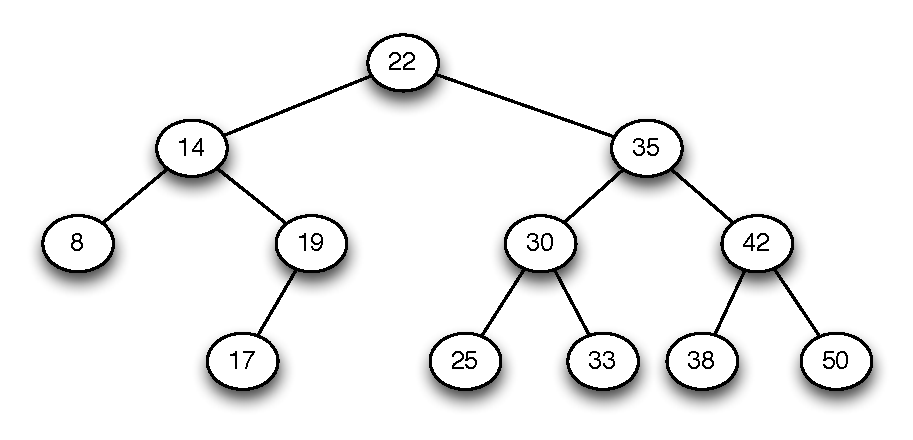
\includegraphics[width=5in]{TreeExerciseGraph.pdf}
}
\end{figure}

\begin{enumerate}

\item What node is at the root of the tree? {\color{red} 22}

\item What are the leaf nodes?  {\color{red} 8, 17, 25, 33, 38, 50}

\item What node is the parent of 42? {\color{red} 35}

\item Are nodes 19 and 30 siblings? {\color{red} No, they do not have the same parent.}

\item What is the height of this tree? {\color{red} 3}

\item What level is node 19? {\color{red} 2}

\item Is this a binary or general tree? {\color{red} It is a binary tree because each node has no more than two children.}

\item If it is a binary tree, is it

\begin{enumerate}

\item a binary search tree? {\color{red} Yes, for each non-leaf node, the left child is $<$ the parent, and the right node is $>$ the parent.}

\item a full binary tree? {\color{red} No, nodes 8 and 19 do not have two children.}

\item a complete binary tree? {\color{red} No, the bottom level is not filled in from left to right.}

\end{enumerate}

\item What are the pre-order, in-order, and post-order traversals of this tree?

\begin{enumerate}

\item Pre-order: {\color{red} 22, 14, 8, 19, 17, 35, 30, 25, 33, 42, 38, 50}

\item In-order: {\color{red} 8, 14, 17, 19, 22, 25, 30, 33, 35, 38, 42, 50}

\item Post-order: {\color{red} 8, 17, 19, 14, 25, 33, 30, 38, 50, 42, 35, 22}

\end{enumerate}

\newpage

\item {Write the expression tree for the following expressions: \\ \\
$m * n * o + p$ \hspace*{3in}$a * (b + c) * d$
}

\begin{figure}[h]
\centerline {
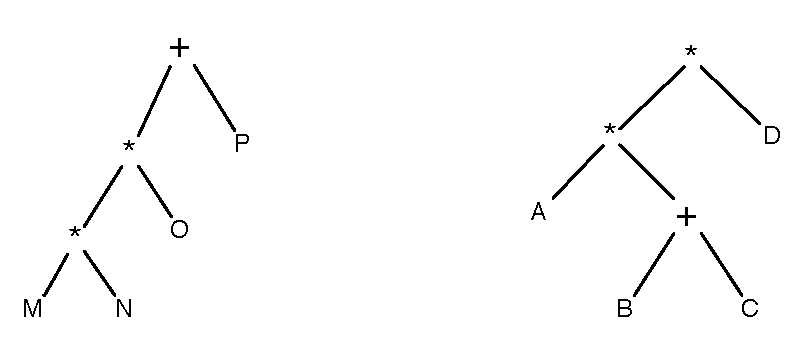
\includegraphics[width=5in]{exp-tree-soln.pdf}
}
%\caption{{\color{red} Solution}}
{\color{red} \caption{Solution}}
\end{figure}

\item What is the height of the shortest binary tree that contains 21 nodes? {\color{red} $\lfloor (lg \; 21) \rfloor = 4$ }

\item Draw the shortest possible binary search tree from the following set of strings 
\begin{center}\{ {\it Ann, Ben, Charles, David, Elizabeth, Fred, Gary, Harold, Isabel, Jay, Kelly} \}\end{center}

\noindent
{\color{red} There are a few different ways, here is one such approach:}

\begin{figure}[h]
\centerline {
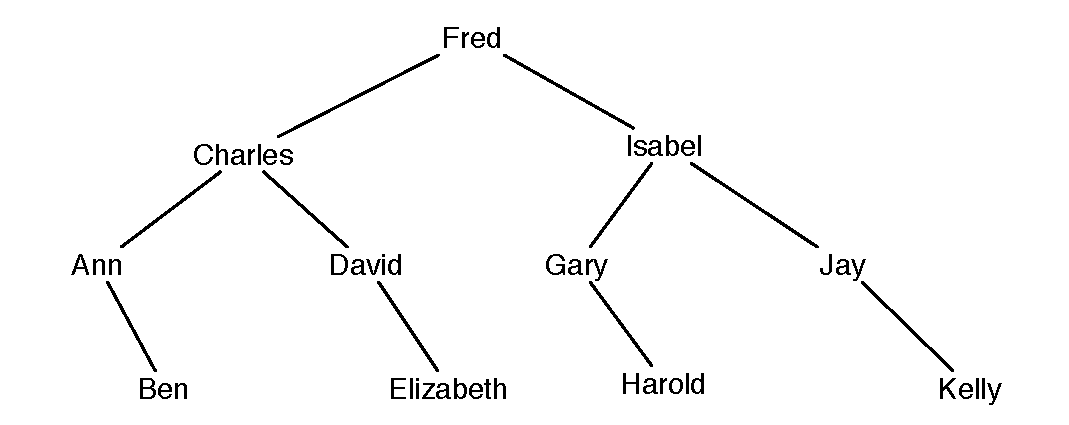
\includegraphics[width=5in]{shortest-bst.pdf}
}
%\caption{{\color{red} Solution}}
{\color{red} \caption{Solution}}
\end{figure}

\newpage



\item At most how many nodes can a binary tree have at level $n$? {\color{red} $2^{n}$}


\item Insert the following values into a binary search tree:
\begin{center} \{ 26, 12, 2, 3, 4, 5, 15, 35, 1 \} \end{center}

\begin{figure}[h]
\centerline {
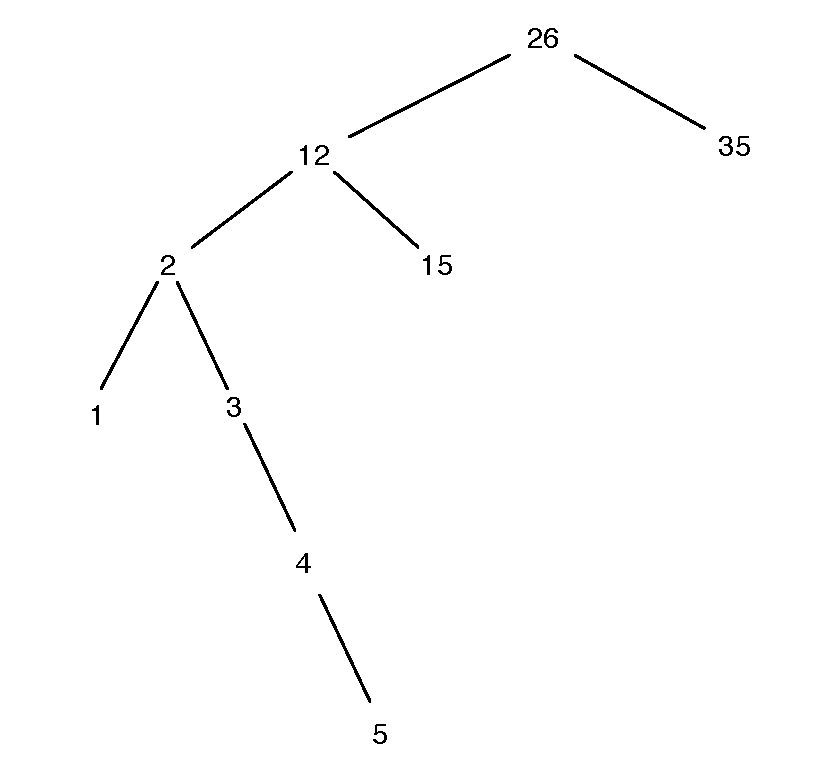
\includegraphics[width=4in]{insert-bst.pdf}
}
%\caption{{\color{red} Solution}}
{\color{red} \caption{Solution}}
\end{figure}

\item Provide three examples from everyday life where a decision tree can be used? 

{\color{red}
\begin{enumerate}

\item Medical diagnosis tool.

\item Stock picking algorithm.

\item Game playing software (i.e. chess.)


\end{enumerate}
}

\end{enumerate}


 \end{document}
